\documentclass[12pt,margin=0.5in]{article}

\usepackage{titlesec}
\usepackage[toc,page]{appendix}
\usepackage{graphicx}
\usepackage[margin=1in]{geometry}
\usepackage{placeins}
\usepackage{caption}
\usepackage{listings}

\lstset{breaklines=true,
		breakatwhitespace=true,
		numbersep=10pt,
		basicstyle=\footnotesize}

\setcounter{secnumdepth}{5}
\setcounter{tocdepth}{5}
\newcommand{\sectionbreak}{\clearpage}
\newcommand{\newparagraph}[1]{\paragraph{#1}\mbox{}\\}
\newcommand{\newoption}[1]{\mbox{}\\{\it #1}}

\graphicspath{{./figs/}{./data/}}

\title{GeoPAT 2.0 user's manual \newline {\normalsize {\bf Notice:} At present this is a very incomplete manual but it has installation instructions.}} 
\date{\today}

\begin{document}
\maketitle
\newpage

\tableofcontents
\newpage

\section{Introduction}
TODO

\section{GeoPAT 2.0 architecture}
TODO
\begin{figure}[h]
%	\centering
	\makebox[\textwidth][c]{\includegraphics[width=1.1\textwidth]{GPAT2.png}}
	\caption{Outline of GeoPAT 2.0 architecture.}
	\label{FIG:GPAT} 
\end{figure}


\subsection{General description}
TODO

\subsection{GeoPAT Modules}

\subsubsection{Signature building}

\newparagraph{gpat\_gridhis}
Creates binary grid of signatures from categorical raster map(s).
\\\\
{\bf Usage:}
\begin{lstlisting}[frame=single]
gpat_gridhis [-lh] -i <file_name> -o <file_name> [-s <signature_name>] [--level=<n>] [-z <n>] [-f <n>] [-n <normalization_name>] [-t <n>]

-i, --input=<file_name>    name of input file (GeoTIFF)
-o, --output=<file_name>   name of output file (GRID)
-s, --signature=<name>     motifel's signature (use -l to list all signatures, default: 'cooc')
--level=<n>                full decomposition level (default: 0, auto)
-z, --size=<n>             motifel size in cells (default: 150)
-f, --shift=<n>            shift of motifels (default: 100)
-n, --normalization=<name> signature normalization method (use -l to list all methods, default: 'pdf')
-l                         list all signatures and normalization methods
-t <n>                     number of threads (default: 1)
-h, --help                 print this help and exit
\end{lstlisting}
{\bf Options:}

\newoption{input}

Defines categorical raster layer(s) which will be used as a source for extracting pattern signature. Layers must be categorical. For Cartesian product method ('prod') there can be more than one input map. Other methods use one map only (the first one provided). In order to provide more than one input map, type multiple input options ("-i map1.tif -i map2.tif" or "--input=map1.tif --input=map2.tif").

\newoption{output}

Output consists of two files: one of them is dataset containing grid of signatures in binary form, the other is a header text file (.hdr extension) containing grid topology and information about the input data parameters. Modifying the header is strongly discouraged. It may cause some calculations to fail. 
Structure of the header is as follows:\\

dim -- number of dimensions of each signature\\
dims -- size of each dimension\\
type -- type of data stored in the grid (integer, float, etc.)\\
at0 -- top left x\\
at1 -- w-e grid resolution\\
at2 -- rotation (0 if grid is north-up)\\
at3 -- top left y\\
at4 -- rotation (0 if grid is north-up)\\
at5 -- n-s grid resolution\\
rows -- number of rows in the grid\\
cols -- number of cols in the grid\\
proj -- projection in wkt style\\
desc -- command used to create the grid

\newoption{size}

Size of a motifel (local calculation window) expressed in the number of pixels. It defines the extent of a local pattern. It is the length of the side of square-shaped block of pixels (motifel). It must be at least 10 and cannot exceed input map size.

\newoption{shift}

Parameter defines the shift between adjacent scenes along the grid in n-s and w-e directions. It describes the density of the output gird and defines new topology of the grid. Formula original\_resolution $\times$ shift = new\_resolution explains how resolution of the original map will be reduced. If shift is set to the same value as 'size', the input map will be simply divided into a grid of non-overlapping motifels. Setting shift to a value smaller than 'size' parameter will result in grid of overlapping motifels. Shift cannot be larger than 'size', and cannot be smaller than 5.

\newoption{signature}

Defines method of calculating signatures of motifels. GeoPAT offers the following methods: 
\begin{itemize}
	\item prod -- Cartesian product of input category lists
	\item cooc -- spatial coocurrence of categories
	\item sdec -- simple 2-level decomposition
	\item fdec -- full decomposition
	\item lbp -- histogram of local binary patterns
	\item lind -- landscape indices vector
	\item linds -- selected landscape indices vector
\end{itemize}
See Appendix \ref{signatures} for details.

\newoption{level}

This option is used only if 'full decomposition' (fdec) is used. It defines the highest level of decomposition. See Appendix \ref{signatures} for details.

\newoption{normalization}

Specifies normalization method used on the signatures. See Appendix \ref{signatures} for details.

\newoption{threads (-t)}

The module is parallel, it can use more than one processing thread in order to speed up calculations. This option specifies how many threads will be used. The default is 1.
\\\\
{\bf Description:}

This module extracts a "grid-of-scenes" (grid of pattern signatures, grid of motifels). The output is a grid of the same spatial extent as the input raster map, but with a different cell size. Each cell in a grid has only one attribute - the signature of its pattern. Pattern is calculated over window centered on that cell and having a user-defined size. Resolution of the output grid equals the resolution of the input raster map multiplied by the shift parameter. A signature of pattern for each scene is stored as numerical vector in binary form. The module outputs a header file (.hdr) containing a topology of a grid-of-scenes and a binary file containing signatures ordered row by row.

As an input module uses categorical raster data in GeoTIFF format. For Cartesian product signature it might be more than one map. Raster maps must be categorical and must be greater than scene size specified by the user. Size defines the size of individual scene for which the histogram is calculated. Shift shows how scenes shift along the grid in n-s and w-e directions. Shift defines the resolution of the new grid. If window size is bigger than shift (recommend), motifels will overlap. If shift and size is equal, windows will not overlap. Shift cannot be greater than size. 

The output grid may be an input to one of the following GeoPAT modules: {\it gpat\_search, gpat\_compare, gpat\_segment, gpat\_segquality, gpat\_grd2txt, and gpat\_globnorm}.

\newparagraph{gpat\_gridts}
{}
\\\\
Usage:
\begin{lstlisting}[frame=single]
gpat_gridts [-nh] -i <file_name> [-i <file_name>]... -o <file_name> [-d <n>]

-i, --input=<file_name>  name of input file(s) (GeoTIFF)
-o, --output=<file_name> name of output file (GRID)
-d, --dimension=<n>      dimension of vector that describes time series element (default: 1)
-n, --normalize          normalize each vector coordinate to [0.0, 1.0] (def
ault: no)
-h, --help               print this help and exit
\end{lstlisting}

\newparagraph{gpat\_pointshis}
Calculates numerical signatures of individual motifels within a raster map.
\\\\
Usage:
\begin{lstlisting}[frame=single]
gpat_pointshis [-lah] -i <file_name> -o <file_name> [-s <signature_name>] [--level=<n>] [-z <n>] [-n <normalization_name>] [-x <double>] [-y <double>] [-d <string>] [--xy_file=<file_name>]

-i, --input=<file_name>    name of input file (GeoTIFF)
-o, --output=<file_name>   name of output file (TXT)
-s, --signature=<name>     motifel's signature (use -l to list all signatures, default: 'cooc')
--level=<n>                full decomposition level (default: 0, auto)
-z, --size=<n>             motifel size in cells (default: 150)
-n, --normalization=<name> signature normalization method (use -l to list all methods, default: 'pdf')
-l                         list all signatures and normalization methods
-x <double>                x coord
-y <double>                y coord
-d, --description=<string> description of the location
--xy_file=<file_name>      name of file with coordinates (TXT)
-a, --append               append results to output file
-h, --help                 print this help and exit
\end{lstlisting}

{\bf Options:}

\newoption{input}

Defines categorical raster map(s) in GeoTIFF format, which will be used as a source for extracting pattern signature. For Cartesian product method ('prod') there can be more than one input map. Other methods use one map only (the first one provided). In order to provide more than one input map, type multiple input options ("-i map1.tif -i map2.tif" or "--input=map1.tif --input=map2.tif").

\newoption{output}

Name of output text file containing signatures. In the output file each line corresponds to a single motifel's signature. Each signature is preceded by its header. A header always consists of: coordinates of the midpoint of motifel (scene), name, number of dimensions, and length of each dimension. Modifying the signature file is strongly discouraged. It may cause some calculations to fail.

\newoption{signature}

Defines method of calculating signatures of motifels. GeoPAT offers the following methods: 
\begin{itemize}
	\item prod -- Cartesian product of input category lists
	\item cooc -- spatial coocurrence of categories
	\item sdec -- simple 2-level decomposition
	\item fdec -- full decomposition
	\item lbp -- histogram of local binary patterns
	\item lind -- landscape indices vector
	\item linds -- selected landscape indices vector
\end{itemize}
See Appendix \ref{signatures} for details.

\newoption{level}

This option is used only if 'full decomposition' (fdec) is used. It defines the highest level of decomposition. See Appendix \ref{signatures} for details.

\newoption{size}

Size of a motifel (scene) for which signature is calculated. Scene is a square centered at the coordinate pair location, while its extent is defined by size. 

\newoption{normalization}

Specifies normalization method used on the signatures. See Appendix \ref{signatures} for details.

\newoption{x}

X coordinate of the midpoint of motifel for which signature will be calculated.

\newoption{y}

Y coordinate of the midpoint of motifel for which signature will be calculated.

\newoption{description}

Description of motifel. It can be name of location, description of pattern, or anything else. If not provided, the default description is "location".

\newoption{xy\_file}

Name of text file with list of pairs of coordinates. This option is very useful for calculating signatures for multiple motifels in a single run.

\newoption{append} (flag)

Append mode. Useful when using coordinate pair mode and scenes are processed one by one (see description below). If the append flag is used and the output file already exists, signatures will be appended at the end of file instead of overwriting it.
\\\\
{\bf Description:}

This module extracts signatures for a scene (motifel) or a collection of scenes defined over square-shaped windows. User provides coordinates of the center of each scene and the size of the scene. The module outputs a list of scene-labeled signatures.
As an input the module uses categorical raster map in GeoTIFF format (or a few maps if user calculates Cartesian product of multiple maps) and coordinates of the center of each scene and size of scenes. The coordinates are in the input map's coordinate system. There are two ways of defining the scenes:

Definition by coordinate pair: 
This is the simplest mode designed for the batch or interactive processing. In this mode, scene is defined by a pair of its midpoint's coordinates ({\it x} and {\it y} options) and scene size parameter ({\it size} option). Only one scene can be processed at once. {\it xy\_file} option is not used in this mode.
If used with append flag (-a), signatures can be calculated one by one and added to the same output file. Additionally, the {\it description} option let user name a scene. This name will be stored in the output file.

Definition by text file:
In this mode, scene midpoint's coordinates are defined in external text file in which each line contains X,Y coordinates and, optionally, name/description using the following syntax: x\_coordinate,y\_coordinate,scene\_name. The name of file with coordinates is provided using {\it xy\_file} option. Extent of a scene is defined by {\it size} parameter. {\it x, y} and {\it description} options are not used in this mode. Example of the content of coordinates file: 
\begin{lstlisting}[frame=single]
1289255,1271313,forest
1306271,1272740,city
1268560,1264726
\end{lstlisting}
If a description is not provided (like in the example above), the program will assign a default name ("location") with id representing the number of line in the coordinate file.

The output signature text file can be used as an input to the following modules: {\it gpat\_search}, {\it gpat\_distmtx}.

\newparagraph{gpat\_pointsts}
{}
\\\\
Usage:
\begin{lstlisting}[frame=single]
gpat_pointsts [-ah] -i <file_name> -o <file_name> [-x <double>] [-y <double>] [-d <string>] [--xy_file=<file_name>]

-i, --input=<file_name>    name of input file (GRID)
-o, --output=<file_name>   name of output file (TXT)
-x <double>                x coord
-y <double>                y coord
-d, --description=<string> description of the location
--xy_file=<file_name>      name of file with coordinates (TXT)
-a, --append               append results to output file
-h, --help                 print this help and exit
\end{lstlisting}

\newparagraph{gpat\_polygon}
Calculates numerical signatures of irregular regions.
\\\\
Usage:
\begin{lstlisting}[frame=single]
gpat_polygon [-lh] -i <file_name> -e <file_name> -o <file_name> [-s <signature_name>] [-n <normalization_name>] [-t <n>]

-i, --input=<file_name>    name of input file (GeoTIFF)
-e, --segments=<file_name> name of input file (GeoTIFF, int)
-o, --output=<file_name>   name of output file (TXT)
-s, --signature=<name>     signature method (use -l to list all methods, default: 'cooc')
-n, --normalization=<name> signature normalization method (use -l to list all methods, default: 'pdf')
-l                         list all signatures and normalization methods
-t <n>                     number of threads (default: 1)
-h, --help                 print this help and exit
\end{lstlisting}

{\bf Options:}

\newoption{input}

Categorical raster map(s) in GeoTIFF format, which will be used as a source for extracting pattern signature. For Cartesian product method ('prod') there can be more than one input map. Other methods use one map only (the first one provided). In order to provide more than one input map, type multiple input options ("-i map1.tif -i map2.tif" or "--input=map1.tif --input=map2.tif").

\newoption{segments}

Categorical raster map in GeoTIFF format which defines spatial division of area of interest into polygonal regions. In this map, regions should be defined as areas of unique ids. Layer must be a raster and its projection, extents and resolution should be identical to the main input map. This layer may be a result of the segmentation module {\it gpat\_segment} or any other categorical map (e.g. map of ids of watersheds).

\newoption{output}

Name of output text file containing signatures. In the output file each line corresponds to a region's signature. Each signature is preceded by its header. A header always consists of: coordinates of the midpoint of region, name, number of dimensions, and length of each dimension. Modifying the signature file is strongly discouraged. It may cause some calculations to fail.

\newoption{signature}

Defines method of calculating signatures of motifels. GeoPAT offers the following methods: 
\begin{itemize}
	\item prod -- Cartesian product of input category lists
	\item cooc -- spatial coocurrence of categories
	\item sdec -- simple 2-level decomposition
	\item fdec -- full decomposition
	\item lbp -- histogram of local binary patterns
	\item lind -- landscape indices vector
	\item linds -- selected landscape indices vector
\end{itemize}
See Appendix \ref{signatures} for details.

\newoption{normalization}

Specifies normalization method used on the signatures. See Appendix \ref{signatures} for details.

\newoption{threads (-t)}

The module is parallel, it can use more than one processing thread in order to speed up calculations. This option specifies how many threads will be used. The default is 1.
\\\\
{\bf Description:}

Module extracts signatures for a collection of irregular regions using the same methods as in {\it gpat\_pointshis} and {\it gpat\_gridhis} module. As an input, apart from categorical raster map from which signatures are calculated, user provides a categorical raster map which defines spatial division of area of interest into polygonal regions. The module outputs a list of polygon labeled-signatures stored in the form of a text file. Output can be transferred to the p.sim.distmatrix for further processing.

The output signature text file can be used as an input to the following modules: {\it gpat\_search}, {\it gpat\_distmtx}.


\subsubsection{Similarity measuring}

\newparagraph{gpat\_search}
Produces similarity maps which show similarity value between query motifels (scenes) and every motifel in the input grid.
\\\\
Usage:
\begin{lstlisting}[frame=single]
gpat_search [-dlh] -i <file_name> [-o <file_name>] -r <file_name> [-m <measure_name>] [--type=Byte/....] [-p <file_name>] [-n <n>] [-t <n>]

-i, --input=<file_name>      name of input file (GRID)
-o, --output=<file_name>     name of output file (TIFF)
-r, --reference=<file_name>  reference data to calculate similarity (TXT)
-d, --description            use description of the reference histogram(s) as name of output file(s)
-m, --measure=<measure_name> similarity measure (use -l to list all measures; default 'jsd')
-l, --list_measures          list all measures
--type=Byte/....             output data type (default: Float64)
-p, --palette=<file_name>    name of the file with colors definition (CSV)
-n, --no_data=<n>            output NO DATA value (default: none)
-t <n>                       number of threads (default: 1)
-h, --help                   print this help and exit
\end{lstlisting}

\newoption{input}

Binary file containing grid of signatures (grid-of-scenes). Grid is mandatory. User has to provide name of grid file (without .hdr extension). Header file is read automatically. Grid is an output from either {\it gpat\_gridhis} or {\it gpat\_gridts} module. Header of the grid will define topology of the output layers. Do not modify header file.

\newoption{reference}

Text file containing one or more signatures of either individual motifels (scenes) or irregular polygons. This option is mandatory. Input text file can be created using {\it gpat\_pointshis}, {\it gpat\_pointsts} or {\it gpat\_polygons} module. The number of outputs depends on the number of scenes in the input scene file. At least one scene is required. Name/description of  will be used to create name of output layer. 

\newparagraph{gpat\_compare}
{}
\\\\
Usage:
\begin{lstlisting}[frame=single]
gpat_compare [-lh] -i <file_name> -i <file_name> -o <file_name> [--type=Byte/....] [-p <file_name>] [-n <n>] [-m <measure_name>] [-t <n>]

-i, --input=<file_name>      name of input files (GRID)
-o, --output=<file_name>     name of output file with similarity (TIFF)
--type=Byte/....             output data type (default: Float64)
-p, --palette=<file_name>    name of the file with colors definition (CSV)
-n, --no_data=<n>            output NO DATA value (default: none)
-m, --measure=<measure_name> similarity measure (use -l to list all measures; default 'jsd')
-l, --list_measures          list all measures
-t <n>                       number of threads (default: 1)
-h, --help                   print this help and exit
\end{lstlisting}

\newparagraph{gpat\_segment}
{}
\\\\
Usage:
\begin{lstlisting}[frame=single]
gpat_segment [-lcgaqh] -i <file_name> -o <file_name> [-v <file_name>] [--size=<n>] [-m <measure_name>] [--lthreshold=<double>] [--uthreshold=<double>] [--swap=<double>] [--minarea=<n>] [--maxhist=<n>] [-t <n>]

-i, --input=<file_name>  name of input files (GRID)
-o, --output=<file_name> name of output file with segments (TIFF)
-v, --vector=<file_name> name of output vector file with segments (SHP)
--size=<n>               output resolution modyfier (default: 1)
-m, --measure=<name>     similarity measure (use -l to list all measures; defult: jsd)
-l, --list_measures      list all measures
--lthreshold=<double>    minimum distance threshold to build areas (default: 0.1)
--uthreshold=<double>    maximum distance threshold to build areas (default: 0.3)
--swap=<double>          improve segmentation by swapping unmatched areas. -1 to skip (default: 0.001)
--minarea=<n>            minimum number of motifels in individual segment (default: 0)
--maxhist=<n>            create similarity/distance matrix for maxhist histograms; leave 0 to use all (default: 200)
-c, --complete           use complete linkage (default is average)
-g, --no_growing         skip growing phase
-a, --no_hierarhical     skip herarhical phase
-q, --quad               quad mode (rook topology)
-t <n>                   number of threads (default: 1)
-h, --help               print help and exit
\end{lstlisting}

\newparagraph{gpat\_distmtx}
{}
\\\\
Usage:
\begin{lstlisting}[frame=single]
gpat_distmtx [-lsh] -i <file_name> -o <file_name> [-m <measure_name>]

-i, --input=<file_name>  name of input file witch signatures (TXT)
-o, --output=<file_name> name of output file (CSV) with similarity matrix
-m, --measure=<name>     similarity measure (use -l to list all measures; default 'jsd')
-l, --list_measures      list all measures
-s, --similarity         output is a similarity matrix
-h, --help               print this help and exit
\end{lstlisting}

\subsubsection{Tools}
\newparagraph{gpat\_grd2txt}
{}
\\\\
Usage:
\begin{lstlisting}[frame=single]
gpat_grd2txt [-h] -i <file_name> -o <file_name>

-i, --input=<file_name>   name of input file (GRID)
-o, --output=<file_name>  name of output file (TXT)
-h, --help                print this help and exit
\end{lstlisting}

\newparagraph{gpat\_globnorm}
{}
\\\\
Usage:
\begin{lstlisting}[frame=single]
gpat_globnorm [-lh] -i <file_name> -o <file_name> [-m <method_name>] [-t <n>]

-i, --input=<file_name>   name of input file (GRID)
-o, --output=<file_name>  name of output file (GRID)
-m, --method=<method_name> 
normalization method (use -l to list all methods, d
efault: '01')
-l, --list_methods        list all methods
-t <n>                    number of threads (default: 1)
-h, --help                print this help and exit
\end{lstlisting}

\newparagraph{gpat\_segquality}
{}
\\\\
Usage:
\begin{lstlisting}[frame=single]
gpat_segquality [-lcqwh] -i <file_name> -s <file name> [-g <file_name>] [-o <file_name>] [-m <measure_name>] [--maxhist=<n>] [-t <n>]

-i, --input=<file_name>     name of input file (GRID)
-s, --segments=<file name>  name of input segmentation map (TIFF)
-g, --inhomogeneity=<file_name> name of output file with segment inhomogeneity (TIF
F)
-o, --isolation=<file_name> name of output file with segment isolation (TIFF)
-m, --measure=<name>        similarity measure (use -l to list all measures; defult: jsd)
-l, --list_measures         list all measures
--maxhist=<n>               create similarity/distance matrix for maxhist histograms; leave 0 to use all (default: 200)
-c, --complete            use complete linkage (default is average)
-q, --quad                quad mode (rook topology)
-w, --no_weight           switch off edge-based weighting in isolation
-t <n>                    number of threads (default: 1)
-h, --help                print help and exit
\end{lstlisting}

\section{Basic workflow paths with examples}

In this section, basic procedures that can be performed using GeoPAT are presented. These are: 
\begin{itemize}
	\item {\bf Search} - search for areas similar to a query,
	\item {\bf Change detection} - comparison of local patterns of two different maps,
	\item {\bf Segmentation} - division of a map into regions of cohesive patterns,
	\item {\bf Clustering} - grouping patterns that are similar to each other.
\end{itemize}
The procedures are explained using workflow schemes, and examples. All the examples of how to process categorical data are shown on a $1400\times 2300$ px ($42\times 69$ km) part of the National Land Cover Dataset (NLCD) covering area around the city of Augusta, GA (Figure \ref{FIG:AUGUSTA}). This area is characterized by high diversity of land cover categories and patterns. Thus it is perfect for various pattern analyzes. 

\begin{figure}[h]
	\centering
	%\includegraphics[width=\textwidth]{Augusta_legend.png}
	\caption{Part of NLCD, covering area around Augusta, GA used in the examples.}
	\label{FIG:AUGUSTA}
\end{figure}

\FloatBarrier

\subsection{Search}

Search functionality enables user to produce a map of similarity. This map shows the level of similarity between a specified motifel (query) and a grid of motifels. The inputs are one or more GeoTIFF raster maps (depending on data and signature type; for more information, see appendix \ref{signatures}), and X,Y coordinates of one or more of points in space. The result is one or more GeoTIFF raster maps which are of the same extents as the grid of motifels specified by user. The number of resulting maps is the same as the number of points provided. The workflows for categorical maps and time series differ.

\subsubsection{Search on categorical maps}
Figure \ref{FIG:SEARCH} presents general workflow path for producing similarity maps using categorical raster data. 

\begin{figure}[h]
	\centering
	\includegraphics[width=\textwidth]{search_scheme.png}
	\caption{Workflow path for search on categorical maps.}
	\label{FIG:SEARCH}
\end{figure}

The first step is to prepare signature files for both query motifels and grid of motifels using two separate modules, {\it gpat\_pointshis} and {\it gpat\_gridhis} respectively. The second step is to use these signature files as inputs to {\it gpat\_search} module in order to produce similarity maps.\\\\
{\bf Example:}

\begin{lstlisting}[numbers=left]
gpat_gridhis -i Augusta2011.tif -o grid -s cooc -z 50 -f 50 -n pdf
gpat_pointshis -i Augusta2011.tif -o query_signatures.txt -s cooc -z 50 -n pdf --xy_file=coordinates.txt
gpat_search -i grid -r query_signatures.txt
\end{lstlisting}

\vspace{5pt}

\vspace{5pt}

\begin{lstlisting}
gpat_pointsts -i grid -o query_signatures.txt --xy_file=coordinates.txt
\end{lstlisting}

do not have to have the same size (but is recommended)

\FloatBarrier

\subsubsection{Search on time series}
TODO
\begin{figure}[h]
	\centering
	\includegraphics[width=\textwidth]{searchts_scheme.png}
	\caption{Workflow path for search on time series.}
	\label{FIG:SEARCHTS}
\end{figure}

\FloatBarrier

\subsection{Change detection}
TODO
\begin{figure}[h]
	\centering
	\includegraphics[width=\textwidth]{compare_scheme.png}
	\caption{Workflow path for change detection.}
	\label{FIG:CHANGE}
\end{figure}

\FloatBarrier

\subsection{Segmentation}
TODO
\begin{figure}[h]
	\centering
	\includegraphics[width=\textwidth]{segment_scheme.png}
	\caption{Workflow path for segmentation.}
	\label{FIG:SEGMENT}
\end{figure}

\FloatBarrier

\subsection{Clustering}
TODO

\subsubsection{Clustering of individual motifels}

\begin{figure}[h]
	\centering
	\includegraphics[width=\textwidth]{cluster_points_scheme.png}
	\caption{Workflow path for clustering of motifels.}
	\label{FIG:CLUSTER_POINTS}
\end{figure}

\begin{figure}[h]
	\centering
	\includegraphics[width=\textwidth]{cluster_pointsts_scheme.png}
	\caption{Workflow path for clustering of time series motifels.}
	\label{FIG:CLUSTER_POINTSTS}
\end{figure}

\FloatBarrier

\subsubsection{Clustering of grid of motifels}

\begin{figure}[h]
	\centering
	\includegraphics[width=\textwidth]{cluster_grid_scheme.png}
	\caption{Workflow path for clustering of grid of motifels.}
	\label{FIG:CLUSTER_GRID}
\end{figure}

\FloatBarrier

\subsubsection{Clustering of segments/predefined irregular regions}

\begin{figure}[h]
	\centering
	\includegraphics[width=\textwidth]{cluster_seg_scheme.png}
	\caption{Workflow path for clustering of segments (regions).}
	\label{FIG:CLUSTER_SEGMENT}
\end{figure}

\FloatBarrier

\begin{appendices}

\section{System requirements}
Windows intaller and Linux binaries provides all necessary components. 
To build GeoPAT 2.0 from the source code the user has to install the GDAL library and compile and install the ezGDAL and SML libraries.

\section{GeoPAT 2.0 installation}

\subsection{Windows installer}
The windows installer works under 64 bit versions of Windows 7, 8.1, and 10.
The installer provides four components:
\begin{itemize}
  \item{GDAL library package}
  \item{ezGDAL and SML libraries}
  \item{GeoPAT 2.0 software}
  \item{Microsoft Visual C 13 runtime libraries (optional)}
\end{itemize}
To start installation process user has to run GPAT20setup.exe.
The setup program should be ran in "Run as administrator" mode.
If an antivirus software is running on the computer, user should 
switch it off temporary for the time of GeoPAT installation.
The installer will create directory for GDAL and GeoPAT and 
copy all necessary files. Optionally, GPAT20setup.exe will
start installer of Microsoft Visual C runtime libraries.
When installation is finished, the user can find "SIL GeoPAT 2.0"
submenu in Windows start menu with "GeoPAT console" and "Uninstall GeoPAT".

The installer for Windows x64 is available at:

\begin{lstlisting}[frame=single]
http://sil.uc.edu/cms/data/uploads/software_data/GPAT20setup.exe
\end{lstlisting}

\subsection{Fedora 25 binary installation}
To install binary version of GeoPAT 2.0, user has to copy contents
of gpat20 directory from gpat20.tar.gz file to /usr/local directory.
The GeoPAT 2.0 binaries require the GDAL package installed on the computer.
The user can install this package using dnf package manager on a Fedora system.

\begin{lstlisting}
dnf install gdal
\end{lstlisting}

The additional requirement is a proper configuration of the libraries path.
The Fedora system should look for libraries in /usr/local/lib.
Sometimes it is necessary to create file local.conf containing following
text: "/usr/local/lib".
The file has to be placed in /etc/ld.so.conf.d directory.

The Fedora 25 x64 binaries are available at:

\begin{lstlisting}[frame=single]
http://sil.uc.edu/cms/data/uploads/software_data/gpat20.tar.gz
\end{lstlisting}

\subsection{Building from source code}

This compilation procedure is focused on Fedora 25
Linux distribution. The user has to modify the procedure
to fit it for a different Linux distribution.

To build GeoPAT 2.0 from the source code the user has to do four following steps:

\begin{itemize}
    \item{Install the developement version of GDAL}
    \item{Build and install the ezGDAL library}
    \item{Build and install the SML library}
    \item{Build and install the GeoPAT 2.0 software}
\end{itemize}

To install the developement version of GDAL, the dnf package manager can be used:

\begin{lstlisting}
dnf install gdal-devel
\end{lstlisting}

To install the ezGDAL library the user has to download the ezGDAL source
code and unpack it. Next, he has to compile the code by calling the following
command in an unpacked source code directory:

\begin{lstlisting}
make
\end{lstlisting}

and to install it

\begin{lstlisting}
make install
\end{lstlisting}

By default the library is placed in /usr/local/lib directory and
include file is placed in /usr/local/include.
The user can change the destination directory by adding the PREFIX parameter.

\begin{lstlisting}
make PREFIX=/my/destination/directory
\end{lstlisting}

When PREFIX is provided, the library is placed in
/my/destination/directory/lib and the include file is placed in
/my/destination/directory/include.

Installation procedure of the SML library is similar. After extraction of the source code of SML, the user should call: "make" and "make install".

The command "make install" should be called using sudo command or in
root user context.

After finishing libraries installation procedure the user has to ensure that
PREFIX/lib is on the library search path.

The last step of installation procedure is a compilation of the GeoPAT 2.0
source code. GeoPAT depends on the GDAL, SML, and ezGDAL libraries.
So, after installing above libraries the user has to unpack, compile
and install GeoPAT code.
The installation procedure is similar to installation procedures of
ezGDAL and SML libraries. PREFIX parameter works in the same way.
"make" commands should be run in the root GeoPAT 2.0 source code
directory.

The source code of GeoPAT 2.0 is available at:

\begin{lstlisting}[frame=single]
http://sil.uc.edu/cms/data/uploads/software_data/gpat2.0src.tar.gz
\end{lstlisting}

The source code of ezGDAL is available at:

\begin{lstlisting}[frame=single]
http://pawel.netzel.pl/data/uploads/software/libezgdal.src.tar.gz
\end{lstlisting}

The source code of SML is available at:

\begin{lstlisting}[frame=single]
http://pawel.netzel.pl/data/uploads/software/libsml.src.tar.gz
\end{lstlisting}

\section{Numerical signatures and normalization methods available in GeoPAT} \label{signatures}
A signature is the numerical description of a motifel

\subsection{Cartesian product}

\subsection{Class co-occurrence histogram}

\subsection{Decomposition histogram}

\subsection{Local binary pattern histogram}

\subsection{Landscape indices vector}

\section{Dissimilarity measures available in GeoPAT}
TODO

\end{appendices}

\bibliographystyle{abbrv}
\bibliography{main}

\end{document}
  
